\documentclass[12pt, twoside, openright]{report} % Fuente a 12pt, formato doble página y chapter a la derecha
\raggedbottom % No ajustar el contenido con un salto de página

% MÁRGENES: 2,5 cm sup. e inf.; 3 cm izdo. y dcho.
\usepackage[
a4paper,
vmargin=2.5cm,
hmargin=3cm
]{geometry}

% INTERLINEADO: Estrecho (6 ptos./interlineado 1,15) o Moderado (6 ptos./interlineado 1,5)
\renewcommand{\baselinestretch}{1.15}
\parskip=6pt

% DEFINICIÓN DE COLORES para portada y listados de código
\usepackage[table]{xcolor}
\definecolor{azulUC3M}{RGB}{0,0,102}
\definecolor{gray97}{gray}{.97}
\definecolor{gray75}{gray}{.75}
\definecolor{gray45}{gray}{.45}

% Soporte para GENERAR PDF/A
\usepackage{etoolbox}
\makeatletter
\@ifl@t@r\fmtversion{2021-06-01}%
 {\AddToHook{package/after/xmpincl}
   {\patchcmd\mcs@xmpincl@patchFile{\if\par}{\ifx\par}{}{\fail}}}{}
\makeatother
\usepackage[a-1b]{pdfx}

% ENLACES
\usepackage{hyperref}
\hypersetup{colorlinks=true,
  linkcolor=black, % enlaces a partes del documento (p.e. índice) en color negro
  urlcolor=blue} % enlaces a recursos fuera del documento en azul

% Añadir pdfs como partes del documento
\usepackage{pdfpages}

% Quitar la indentación de principio de los párrafos
\setlength{\parindent}{0em}

% EXPRESIONES MATEMÁTICAS
\usepackage{amsmath,amssymb,amsfonts,amsthm}

\usepackage{txfonts} 
\usepackage[T1]{fontenc}
\usepackage[utf8]{inputenc}

% Insertar gráficas y fotos
\usepackage{tikz}
\usepackage{pgfplots}

\usepackage[spanish, es-tabla]{babel} 
\usepackage[babel, spanish=spanish]{csquotes}
\AtBeginEnvironment{quote}{\small}

% diseño de PIE DE PÁGINA
\usepackage{fancyhdr}
\pagestyle{fancy}
\fancyhf{}
\renewcommand{\headrulewidth}{0pt}
\fancyfoot[LE,RO]{\thepage}
\fancypagestyle{plain}{\pagestyle{fancy}}

% DISEÑO DE LOS TÍTULOS de las partes del trabajo (capítulos y epígrafes o subcapítulos)
\usepackage{titlesec}
\usepackage{titletoc}
\titleformat{\chapter}[block]
{\large\bfseries\filcenter}
{\thechapter.}
{5pt}
{\MakeUppercase}
{}
\titlespacing{\chapter}{0pt}{0pt}{*3}
\titlecontents{chapter}
[0pt]                                               
{}
{\contentsmargin{0pt}\thecontentslabel.\enspace\uppercase}
{\contentsmargin{0pt}\uppercase}                        
{\titlerule*[.7pc]{.}\contentspage}                 

\titleformat{\section}
{\bfseries}
{\thesection.}
{5pt}
{}
\titlecontents{section}
[5pt]                                               
{}
{\contentsmargin{0pt}\thecontentslabel.\enspace}
{\contentsmargin{0pt}}
{\titlerule*[.7pc]{.}\contentspage}

\titleformat{\subsection}
{\normalsize\bfseries}
{\thesubsection.}
{5pt}
{}
\titlecontents{subsection}
[10pt]                                               
{}
{\contentsmargin{0pt}                          
  \thecontentslabel.\enspace}
{\contentsmargin{0pt}}                        
{\titlerule*[.7pc]{.}\contentspage}  

% DISEÑO DE TABLAS.
\usepackage{multirow} % permite combinar celdas 
\usepackage{caption} % para personalizar el título de tablas y figuras
\usepackage{floatrow} % utilizamos este paquete y sus macros \ttabbox y \ffigbox para alinear los nombres de tablas y figuras de acuerdo con el estilo definido. Para su uso ver archivo de ejemplo 
\usepackage{array} % con este paquete podemos definir en la siguiente línea un nuevo tipo de columna para tablas: ancho personalizado y contenido centrado
\newcolumntype{P}[1]{>{\centering\arraybackslash}p{#1}}
\DeclareCaptionFormat{upper}{#1#2\uppercase{#3}\par}

% Diseño de tabla para ingeniería
\captionsetup[table]{
  format=hang,
  name=Tabla,
  justification=centering,
  labelsep=colon,
  width=.75\linewidth,
  labelfont=small,
  font=small,
}

% DISEÑO DE FIGURAS.
\usepackage{graphicx}
\graphicspath{{img/}} %ruta a la carpeta de imágenes

% Diseño de figuras para ingeniería
\captionsetup[figure]{
  format=hang,
  name=Fig.,
  singlelinecheck=off,
  labelsep=colon,
  labelfont=small,
  font=small    
}

% NOTAS A PIE DE PÁGINA
\usepackage{chngcntr} % Para numeración continua de las notas al pie
\counterwithout{footnote}{chapter}

% LISTADOS DE CÓDIGO
% soporte y estilo para listados de código. Más información en https://es.wikibooks.org/wiki/Manual_de_LaTeX/Listados_de_código/Listados_con_listings
\usepackage{listings}

% definimos un estilo de listings
\lstdefinestyle{estilo}{ frame=Ltb,
  framerule=0pt,
  aboveskip=0.5cm,
  framextopmargin=3pt,
  framexbottommargin=3pt,
  framexleftmargin=0.4cm,
  framesep=0pt,
  rulesep=.4pt,
  backgroundcolor=\color{gray97},
  rulesepcolor=\color{black},
  %
  basicstyle=\ttfamily\footnotesize,
  keywordstyle=\bfseries,
  stringstyle=\ttfamily,
  showstringspaces = false,
  commentstyle=\color{gray45},     
  %
  numbers=left,
  numbersep=15pt,
  numberstyle=\tiny,
  numberfirstline = false,
  breaklines=true,
  xleftmargin=\parindent
}

\captionsetup[lstlisting]{font=small, labelsep=period}
% fijamos el estilo a utilizar 
\lstset{style=estilo}
\renewcommand{\lstlistingname}{\uppercase{Código}}

\pgfplotsset{compat=1.17} 
%-------------
% DOCUMENTO
%-------------

\begin{document}
\pagenumbering{roman} % Se utilizan cifras romanas en la numeración de las páginas previas al cuerpo del trabajo

%----------
% PORTADA
%---------- 
\begin{titlepage}
	\begin{sffamily}
		\color{azulUC3M}
		\begin{center}
			\begin{figure}[H] %incluimos el logotipo de la Universidad
				\makebox[\textwidth][c]{
\includegraphics[width=16cm]{Portada_Logo.png}}
			\end{figure}
			\vspace{2.5cm}
			\begin{Large}
				Grado en Ingeniería Informática\\
				2021-2022\\
				\vspace{2cm}
				\textsl{Apuntes}\\
				\bigskip
			\end{Large}
			{\Huge Redes de Neuronas Artificiales}\\
			\vspace*{0.5cm}
			\rule{10.5cm}{0.1mm}\\
			\vspace*{0.9cm}
			{\LARGE Jorge Rodríguez Fraile\footnote{\href{mailto:100405951@alumnos.uc3m.es}{Universidad: 100405951@alumnos.uc3m.es}  |  \href{mailto:jrf1616@gmail.com}{Personal: jrf1616@gmail.com}}}\\
			\vspace*{1cm}
		\end{center}
		\vfill
		\color{black}
		
\includegraphics[width=4.2cm]{img/creativecommons.png}\\
		Esta obra se encuentra sujeta a la licencia Creative Commons\\ \textbf{Reconocimiento - No Comercial - Sin Obra Derivada}
	\end{sffamily}
\end{titlepage}

%----------
% ÍNDICES
%---------- 

%--
% Índice general
%-
\tableofcontents
\thispagestyle{fancy}

%--
% Índice de figuras. Si no se incluyen, comenta las líneas siguientes
%-
\listoffigures
\thispagestyle{fancy}

%--
% Índice de tablas. Si no se incluyen, comenta las líneas siguientes
%-
\listoftables
\thispagestyle{fancy}

%----------
% TRABAJO
%---------- 

\pagenumbering{arabic} % numeración con múmeros arábigos para el resto de la publicación  


%----------
% COMENZAR A ESCRIBIR AQUI
%---------- 

\chapter{Información}

\section{Profesores}
\begin{quote}
	Magistral: Isasi Viñuela, isasi@ia.uc3m.es

	Prácticas: José María Valls, jvalls@inf.uc3m.es

	Inés M. Galván, igalvan@inf.uc3m.es (de baja)
\end{quote}

\section{Objetivos}
\begin{itemize}
	\item “Transmitirnos su entusiasmo por las redes neuronales”, darnos la posibilidad de acceder más fácilmente a este mundo.
	\item Entender que subyace sobre estas redes y el método científico.
	\item Estudiar los diferentes modelos de redes.
	\item Describir las diferentes áreas de aplicabilidad de las redes de neuronas.
	\item Resolver problemas con redes de neuronas.
	\item Analizar las ventajas e inconvenientes de neuronas.
	\item Analizar las ventajas e inconvenientes de cada uno de los modelos de redes desde una perspectiva aplicada.
	\item Diseñar un conjunto de experimentos para la resolución de problemas.
\end{itemize}

\section{Sistema de evaluación}
\begin{itemize}
	\item 60 \% Evaluación continua
	      \begin{itemize}
		      \item 20 \% Practica 1. Trata de resolver un problema de regresión, estimar un número real, y se divide en dos partes:
		            \begin{itemize}
			            \item  Modelo lineal (ADALINE) determinando los coeficientes, este caso tenemos programarlo nosotros en nuestro lenguaje de preferencia.
			                  Se nos proporcionan unos datos de prueba para cuando lo estemos programando salga un error muy pequeño, de esta manera sabemos si lo hacemos bien. Las de prueba son 3 atributos, pero los reales son de 8.
			            \item  No lineal (Perceptrón multicapa), presentando una memoria de unas 8 páginas en forma de artículo.
			                  Para esta parte se nos dará un script en R, no hay que programarlo, pero hay que realizar muchas pruebas para ver los resultados (errores).
		            \end{itemize}
		      \item 20 \% Practica 2. Habrá que modificar scripts de Python, también ser usará Google Colab.
		            \begin{itemize}
			            \item Parte 1: Problema de clasificación que resolveremos con Perceptrón multicapa.
			            \item Parte 2: Problema de clasificación con imágenes usando Deep Learning.
		            \end{itemize}
		      \item 20 \% Prueba parcial, de las prácticas (a principios de noviembre).
	      \end{itemize}
	\item 40 \% Examen final, se realizarán cuestiones teórico-prácticas, pudiendo incluir preguntas sobre las prácticas.
	      \begin{itemize}
		      \item Se puede emplear material.
		      \item No hay nota mínima
	      \end{itemize}
\end{itemize}

Para la bibliografía se empleará en los primeros temas el libro escrito por los profesores (Redes de Neuronas Artificiales. Un enfoque práctico, 2004), pero para el resto de los temas sobre todo Deep Learning (Redes Neuronales \& Deep Learning de Fernando Bernal, 2018).

\chapter{Practica 1}
\section{Preparación de Datos}
\subsection{Los datos}
Variables, datos o patrones de entrada y de salida deseada de la red, que solo trabajan con atributos numéricos y cuando no son numéricos se discretizan para que pasen a ser numéricos.

\textbf{Supervisado:} Hay una salida que es lo que buscamos determinar.

\textbf{No supervisado:} Tratamos de agrupar o buscar una determinada estructura en los datos, no hay salida.

\subsection{Transformación de los datos}
\textbf{Normalización de datos:} Se emplea en los casos en los que los valores entre los atributos con muy dispares (ej. 0.1 y 10) lo que provocaría que al realizar operaciones entre ellos dieran valores que dependen mucho más de un atributo que otro. Los valores se ajustan al rango de 0 y 1.

$$ValorNormalizado_i=\frac {Valor_i-ValorMinimo_i} {ValorMaximo_i-ValorMinimo_i}$$

\textbf{Aleatorización de los datos:} Se altera el orden las instancias de manera que se evita cualquier sesgo a la hora de entrenar el modelo.

\textbf{Eliminación de  atributos irrelevantes:} Nosotros no lo haremos, pero este nos permite eliminar la información que no aporta nada y entorpece el entrenamiento.

\textbf{Reducción dimensionalidad:} Se realizan las técnicas de reducción de dimensionalidad, que bien seleccionan un subconjunto de atributos, bien transforman los datos de entrada en otro conjunto de mayor dimensión.

\subsection{Evaluación de una red de Neuronas}
\textbf{Separación del conjunto de entrenamiento y test:} Se separa un conjunto de instancias que se emplearan solo para el entrenamiento y otro que se utilizara solo para evaluar el modelo, el conjunto de test. Esto permitirá detectar si el entrenamiento que estamos haciendo se está sobreajustando, haciendo que no generalizase adecuadamente.
\pagebreak

\textbf{Validación cruzada:} Consiste en dividir los datos en una serie de conjuntos de igual tamaño. Con estos conjuntos se va entrenando, dejando uno fuera en todo momento para utilizarlo como test. Esto nos permite evaluar el error haciendo la media de todos los errores obtenidos con los modelos, siendo este valor error del modelo que se obtienen entrenando con todas las instancias.

\textbf{Validación cruzada estratificada:} Se dividen de igual las instancias en conjuntos de igual tamaño. En este caso lo que se hace es que haya en cada conjunto la misma proporción de instancias con cada clase con respecto al total. Todos tendrán la misma proporción de instancias de una clase que los otros del total.
Lo que se hace es separar las instancias por la clase, de estos conjuntos generados se divide cada uno en el número de conjuntos de validación cruzada, de esta manera en cada uno de los conjuntos que vamos a generar vamos cogiendo uno conjunto de cada una de las clases.

\textbf{Medida de evaluación}
\begin{itemize}
	\item \textbf{En regresión:} Error absoluto medio (Mean Absolute Error) es la media del valor absoluto de la diferencia de la salida y el deseado. Error cuadrático medio (Mean Square Error) es igual al anterior, pero en vez de valor absoluto la diferencia se pone al cuadrado.
	      $$MAE=\frac 1 N \sum^N_{i=1} |s_i-d_i| \quad MSE=\frac 1 N \sum^N_{i=1} (d_i-s_i)^2$$
	      Acaba cuando el error medio o el cuadrático es aceptable. También por una visualización gráfica de las salidas deseadas y las salidas de la red.
	\item \textbf{En clasificación:} Lo más habitual es evaluar la calidad de la red basándonos en su precisión predictiva (\% de aciertos), la proporción de aciertos sobre el total de instancias.

	      Acaba cuando el porcentaje de aciertos es alto, teniendo en cuenta que debe ser mayor que la probabilidad de que acierte aleatoriamente (como si tirase una moneda) y las clases están equilibradas (porque si siempre da una clase podría tener un buen porcentaje de acierto dando un valor constante).

	      \textbf{Matriz de confusión:} Representa la cantidad de instancias según lo estimado y lo correcto, de manera que se pueda ver los que han sido estimados según TP, FN, FP o TN. Los datos correctamente clasificados están en la diagonal, los incorrectos fuera de ella. Se emplean otras medidas como son:
	      \begin{itemize}
		      \item El porcentaje de aciertos total es $\frac {TP+TN} {TP+TN+FN+FP}$
		      \item El porcentaje de aciertos de + es: $\frac {TP} {TP+FN}$
		      \item El porcentaje de aciertos – es: $\frac {TN} {FP+TN}$
	      \end{itemize}

\end{itemize}

\subsection{Anotaciones Practica 1}
A la hora de normalizar hacerlo sobre el total de los datos, no solo sobre los de entrenamiento.
Aleatorizarlos.
Separar las instancias en 70 15 15.

En la parte de programar los vectores de pesos y umbrales, si se hace un vector con los pesos y el umbral, tener en cuenta que al hacer el producto cartesiano el de entrada debe tener un 1 para el umbral. $[x_1 \; x_2 \; x_3 \; 1]$ con $[w_1 \; w_2 \; w_3 \; \sigma]$

\chapter{Tema 1: Introducción}
El objeto de la IA es la construcción de sistemas inteligentes.

\textbf{Sistema Inteligente:} Dispositivo físico o lógico con capacidades propias de los humanos como tomar decisiones, resolución de problemas o el aprendizaje.

Partiremos de la base, por lo que el primer paso serán organismos más pequeños, pero el objetivo es alcanzar la capacidad humana y llegar a sustituirnos.

Áreas
\begin{itemize}
	\item \textbf{Simbólica (Top-down):} Diseñar componentes del sistema inteligente donde el comportamiento es programado por nosotros para que él sea capaz de razonar y aprender. Se emplea en búsqueda y optimización
	\item \textbf{Subsimbólica (Bottom-up):} Se programa lo básico y lo dejamos interactuar para ver si llega a un punto adecuado. No programamos el comportamiento, sino las partes base y miramos a ver como se relaciona y si lo resuelve.
\end{itemize}

Las \textbf{Redes de Neuronas} se encuentran en la IA subsimbólica, tratan de emular los sistemas neuronales biológicos. Se ha estado durante décadas detrás de la construcción de algoritmos capaces de procesar la información de la misma manera que lo hace el cerebro humano.

Se caracterizan por tener la \textbf{propiedad de aprender} a partir de ejemplos.

Tratan \textbf{información numérica}, si se puede discretizar bien, si no se emplean otros métodos.

En la actualidad existe un gran número de arquitecturas diferentes de redes de neuronas artificiales, además este progreso ha sido posible por la capacidad de cómputo, esos procesos son muy costosos.

Algunas \textbf{áreas de aplicación}:
\begin{itemize}
	\item Reconocimiento de patrones (imagen, voz, caracteres)
	\item Compresión y análisis de datos.
	\item Robótica.
	\item Medicina.
	\item Predicción de series temporales.
\end{itemize}

Las redes de neuronas no permiten abordar problemas de: Aproximación, Predicción, Clasificación, Agrupación.

\textbf{Otras técnicas de IA que se pueden emplear} para estos problemas son:
\begin{itemize}
	\item Máquinas de Vectores de Soporte (Vapnik, 1995)
	\item Gradient Boosting (Friedman, 2002)
	\item Random Forest (Breiman, 2001)
	\item K-medias (agrupación) (MacQueen, 1967)
\end{itemize}

\textbf{Ventajas}
\begin{itemize}
	\item Son fáciles de utilizar y diseñar, la parte difícil es acertar.
	\item Capacidad de aprender a partir de ejemplos.
	\item Tolerancia al ruido en los ejemplos, es muy tolerante a fallos, incluso a la perdida de unas pocas neuronas.
	\item Diversidad de las áreas de aplicación, teniendo datos se puede aplicar en problemas de cualquier área aunque no seamos expertos en la misma.
\end{itemize}

Desde la aparición de las redes sociales y móviles las compañías han recogido muchísimos datos que han posibilitado el entrenamiento de  redes en muchas áreas.

\textbf{Problemas específicos de las RNA}
\begin{itemize}
	\item Tiempo de aprendizaje, requiere mucha capacidad de cómputo y son lentos.
	\item Determinación de los hiperparametros, como el número de neuronas, ciclos, etc.
	\item No se pueden explicar los resultados, como una caja negra por lo que se están diseñando redes cuyo propósito es explicar.
\end{itemize}

\section{Historia}
Comienza en \textbf{1940} con estudios en la neurocirugía, al descubrir la neurona, se empezó a ver el funcionamiento del cerebro y se vio que funcionaba por señales eléctricas. A raíz de esto se hicieron modelos computaciones basados en lo que se conocía, se crearon para puertas lógicas inicialmente (con pesos fijos). El primer modelo fue de S. McCulloch y W. Pitts, que permitía pesos que se ajustaban, pero no se aprendían.

F. Rosenblatt en \textbf{1957} diseñó el Perceptrón que tenía un proceso para calcular los pesos según las entradas, en esos momentos la entrada era binaria.

B. Widrow y M. Hoff en \textbf{1960} diseñaron el \textbf{ADALINE} que permitía entradas no binarias.

Faltaban neuronas por falta de hardware, pero se pensaba que ya estaba todo hecho.

M. Minsky y S. Papert con el \textbf{libro “Perceptrón”} en \textbf{1969} rompieron el pensamiento de que todo estaba hecho con el \textbf{XOR Problem}, en el que no existe un único plano que represente la logia de la puerta XOR. Este problema inició la Época oscura (“AI Winter”).

D. Rumelhart, G. Hinton y R. William en \textbf{1986} solucionaron el problema XOR con más de 1 capa en el perceptrón, lo que da origen al \textbf{Perceptrón Multicapa y la Retropropagación.}

V. Vapnik y C. Cortes en \textbf{1995} desarrollaron las Máquinas de Vectores de Soporte (SVM) que están relacionados con problemas de clasificación y regresión.

En el año \textbf{2006} ya había capacidad de cómputo, se podía dar más profundidad con un mayor número de capas \textbf{Redes de Neuronas Profundas}, pero no se avanzó mucho en la teoría, se basaba en lo que había dicho Rumelhart.

\section{Fundamentos biológicos}
El \textbf{Sistema nervioso} es un conjunto de células especializadas en la conducción de señales eléctricas. Capta estímulos del entorno o internos, procesa la información y genera respuestas diferentes según la situación. No todos son igual de complejos, la estructura es lo que varía, pero todos están compuestos por los mismos componentes.

El \textbf{Cerebro} es el órgano principal del Sistema Nervioso. Se encarga de regular y mantener cada función vital del cuerpo, y es el órgano donde reside la mente y la conciencia del individuo. Existen distintas áreas, cada una más sofisticada para una serie de tareas (como puede ser la motora, sensoria, etc.), pero todas son importantes para el individuo.
\begin{itemize}
	\item Está formado por $10^{11}$ células, llamadas neuronas, interconectadas entre sí (cada una a otras 1000-10000 $10^{15}$) y forman una densa red.
\end{itemize}

Las neuronas se comunican a través de \textbf{impulsos eléctricos de corta duración, que se transmiten a través de las sinapsis}.

El impulso se propaga a través del axón, y es recibido por la dendrita (ramificaciones de la neurona que buscan axones) de la célula receptora.

El \textbf{Axón} (una sola por neurona) se ramifica, y puede propagar una misma señal a cientos de dendritas de células diferentes. Contiene unas vesículas que contienen los neurotransmisores, que al liberarse se comunican con la neurona inmediata por medio de la sinapsis. La señal que se propaga es única y es recibida por todas las células conectadas.

Las \textbf{Dendritas} reciben multitud de señales diferentes, algunas excitatorias y otras inhibitorias.
\pagebreak

Cuando el impulso llega a la neurona pre-sináptica, abre los canales de ion cálcico que liberan los neurotransmisores que son captados por los receptores de la neurona post-sináptica que abren o cierran los canales iónicos de la dendrita generando potenciales eléctricos que permiten la propagación de la señal hacia el soma de la célula. Se va despolarizando al recibir estímulos eléctricos, cuando supera un umbral se dispara un potencial de acción.

\textbf{Son elementos no lineales:} Si se supera un umbral, se produce una señal de activación

El sistema nervioso funciona como una enorme malla que propaga señales electroquímicas de unas células a otras, modificando sucesivamente la concentración de iones de las sinapsis.

Robustez y tolerancia a fallos

Adaptación y plasticidad

Manejar información: inconsistente, difusa y con ruido

Una \textbf{red artificial (ResNet152) puede llegar a los 60 millones de sinapsis} (diez millones de veces más pequeña), todavía estamos lejos.

\section{Neurona artificial}
Trata de imitar las características generales de las neuronas.
\begin{figure}[H]
	\ffigbox[\FBwidth]
	{\caption{Comparación neurona bilógica y neurona artificial}}
	{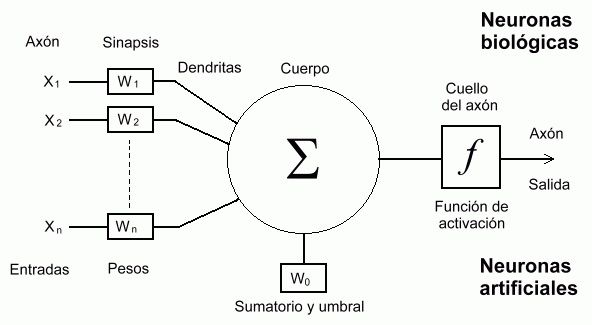
\includegraphics[scale=.8]{neurona-vs-perceptron.jpg}}
\end{figure}

Las \textbf{dendritas funcionan como las entradas} en la neurona, el \textbf{axón como la salida} y la \textbf{densidad de la sinapsis para que pase mejor el impulso serían los pesos}.

En cuanto al \textbf{potencial de acción (cuando supera el umbral) se simula con una función de activación} no lineal. Se utiliza un \textbf{umbral para poder ajustar esta función}.

Cada neurona está caracterizada por un estado interno denominado nivel de activación:
\begin{itemize}
	\item Discreto: Desactivado o Activado, S=0,1.
	\item Continuo: S=[0,1].
\end{itemize}

\textbf{Función de activación:} permite cambiar el nivel de activación a partir de las señales de entrada.

Las señales de entrada se combinan entre sí, generando la entrada total.

\textbf{Tipos de funciones de activación:}
\begin{figure}[H]
	\ffigbox[\FBwidth]
	{\caption{Tipos de funciones de activación}}
	{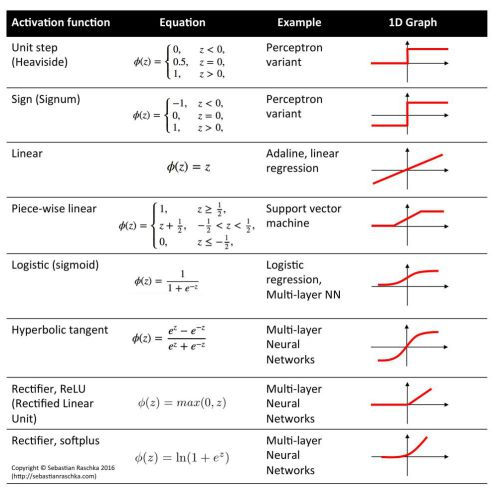
\includegraphics[scale=.8]{tipos-fun-act.jpg}}
\end{figure}

Las que nosotros emplearemos con la Sigmoide, Tangente hiperbólica y la ReLU (Rectified Linear Unit, es lineal a partir de 0).

Excepto la función lineal estas propagan la señal de manera no lineal.
\pagebreak

\subsection{Modelo computacional}
\textbf{Componentes}
\begin{itemize}
	\item Conjunto de unidades de proceso o neuronas artificiales.
	\item Conexiones entre las unidades.
	\item Regla de propagación, para propagar las entradas hacia la salida de la red.
	\item Regla de aprendizaje para modificar los pesos de las conexiones.
\end{itemize}

Tiene una arquitectura en forma de capas (entrada, ocultas y salida) que se propaga hacia delante (izq. a dch.).

Las capas ocultas son las que realizan el procesamiento, la entrada y salida solo se encargan de recibir y sacar los datos de la red.

Las conexiones van de una capa a la inmediata siguiente, no saltan capas o retroceden (todavía no). Todas las neuronas de una capa están conectadas con cada una de la capa anterior y posterior (full connected).

El aprendizaje consiste en ajustar los pesos de tal manera que pueda resolver el problema de manera eficaz.

\subsection{Aprendizaje}
Tratamos de que al pasar un patrón (serie de datos de entrada) nos dé la salida correspondiente, para esto cuando falla hay que ajustar los pesos y umbral.

Se realiza a partir de un conjunto de ejemplos o muestras conocidas, que llamaremos Conjunto de entrenamiento. Se debe disponer de una cantidad significativa y representativa de ejemplos para realizar un buen aprendizaje, suficientes ejemplos y que cubran la variedad de salidas.

\textbf{Proceso:}
\begin{enumerate}
	\item Introducir progresivamente los ejemplos de aprendizaje.
	\item Modificar los pesos siguiendo una ley o ecuación de aprendizaje.
	\item Cuando se han introducido todos se ha completado una iteración. Ahora se comprueba si se cumple cierto criterio de convergencia y si no se cumple, se repite el proceso.
\end{enumerate}
\pagebreak

La modificación de los pesos puede ocurrir después de introducir cada patrón (lo habitual) o después de introducir todos los patrones (o un lote de estos, permite acelerar el proceso y se usa en Redes Convolucionales).

En cuanto a la finalización del aprendizaje se hace en función de un criterio de convergencia que puede ser que el error sea menor que un valor dado (puede no llegar a ocurrir) o que los pesos dejen de sufrir modificaciones y el error se estabilice.

\textbf{Modelos de aprendizaje:}
\begin{itemize}
	\item \textbf{Aprendizaje supervisado:} Se conoce la salida de los ejemplos de aprendizaje. Utiliza un proceso externo para determinarlo. Conocer el resultado nos permite manejar el error cometido y guiar el aprendizaje
	\item \textbf{Aprendizaje no supervisado:} No se conoce la salida de los ejemplos. Permite detectar características de los datos, agruparlos o reducir la dimensionalidad. Se reajustan automáticamente los pesos y autoorganiza la información.
	\item \textbf{Aprendizaje por refuerzo:} Se aprende por prueba y error guiado por una recompensa si lo hace bien. No existe medida de error, solo si lo ha habido.
\end{itemize}

\subsection{Validación}
El modelo resultante debe ser capaz de responder de forma adecuada ante datos desconocidos. Meter datos no conocidos y usarlos solo para evaluar (no aprender) si el modelo es bueno.

El conjunto de datos disponibles se divide en subconjuntos de:
\begin{itemize}
	\item \textbf{Entrenamiento:} Usado para ajustar el valor de los pesos.
	\item \textbf{Validación (no siempre se utiliza este conjunto):} Usado para determinar los hiperparámetros de la red y detener el aprendizaje. Permite detectar sobre ajuste.
	\item \textbf{Test:} Usado para medir la capacidad de generalización de la red. Se utiliza este segundo no conocido porque no es conocido y no se ha utilizado previamente (ni entrenar, ni para el entrenamiento) son verdaderamente nuevos para el modelo.
\end{itemize}

Los conjuntos de validación y test deben ser Independientes del aprendizaje, Significativos y representativos.

\textbf{Sobreajuste (overfitting):} La red se ha sobreajustado a los ejemplos de entrenamiento, deja de generalizar bien.
\pagebreak

\subsection{Taxonomía}
Redes Feedforward supervisadas: Conexiones hacia delante y aprendizaje supervisado.
\begin{itemize}
	\item Perceptrón simple, Adaline, Perceptrón Multicapa, Redes de Base Radialy Redes Convolucionales.
\end{itemize}

Redes no supervisadas
\begin{itemize}
	\item Kohonen y ART.
\end{itemize}

Redes recurrentes: Conexiones en todas las direcciones
\begin{itemize}
	\item Solo unas pocas conexiones recurrentes: Red de Jordan, Red de Elman
	\item Totalmente recurrentes: Backpropagation a través del tiempo, Long short-term memory.
\end{itemize}

\subsection{Diferencia de las RNA y Biología}
Estamos muy lejos todavía, el cerebro tiene 10 millones más de sinapsis y no necesita capas de neuronas. Siempre está aprendiendo (y olvidando).

El cerebro trabaja de manera asíncrona (se ajusta cuando lo necesita) y las RNA son síncronas (cuando se actualizan los pesos lo hacen todos a la vez).

Las RNA para aprender usan el descenso de gradiente, pero del cerebro no se conoce.
\pagebreak

\section{Primeros modelos}
\subsection{Células de McCulloch-Pitts}
\begin{figure}[H]
	\ffigbox[\FBwidth]
	{\caption{Estructura de Célula de McCulloch-Pitts}}
	{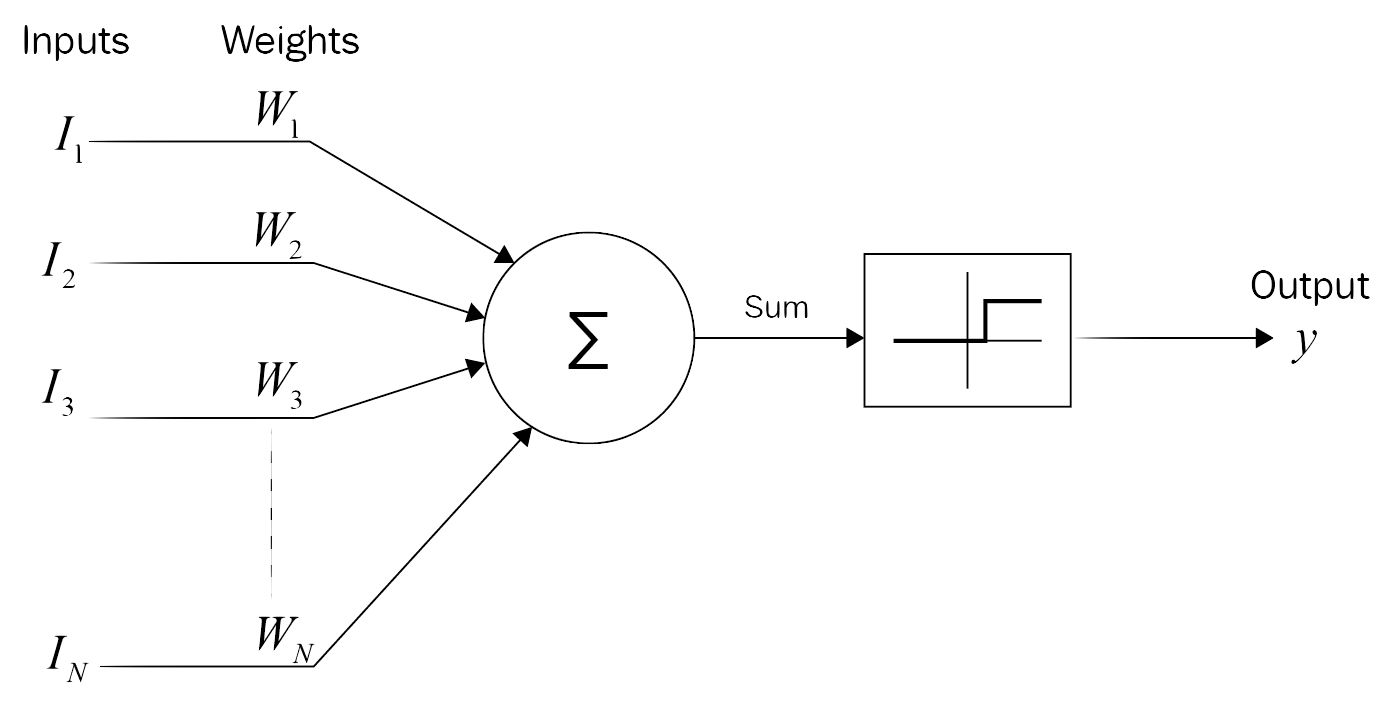
\includegraphics[scale=.25]{McCulloch-Pitts.jpg}}
\end{figure}
Consiste en unas entradas que tienen asignado manualmente un peso cada una de las que se hace el sumatorio de la entrada por el peso, este resultado se pasa por una función de activación no lineal y se obtiene la salida.
$$y=f\left(\sum_{i=1}^n I_i w_i\right) \quad f (x) = \begin{cases}1 & \textit{si}\quad  x> 0\\0 & \textit{en caso contrario}\end{cases}$$
En este momento hablamos de células individuales, no de redes.

\subsubsection{Limitaciones}
Se puede simular cualquier puerta lógica. Uniendo las puertas lógicas, se puede representar cualquier función.

El problema es el diseño de la red, que requiere determinar la arquitectura y los pesos. Se necesita un mecanismo para que determine los pesos automáticamente, es muy pesado hacerlo a mano.

El perceptrón son un conjunto de células de McCulloch-Pitts, con una sola capa, y cuyos pesos pueden ser determinados a partir de los ejemplos de los que se disponga.
\pagebreak

\subsection{Perceptrón}
Tiene una estructura similar a las células de McCulloch-Pitts, pero además de los pesos hay un umbral.
\begin{figure}[H]
	\ffigbox[\FBwidth]
	{\caption{Estructura del Perceptrón}}
	{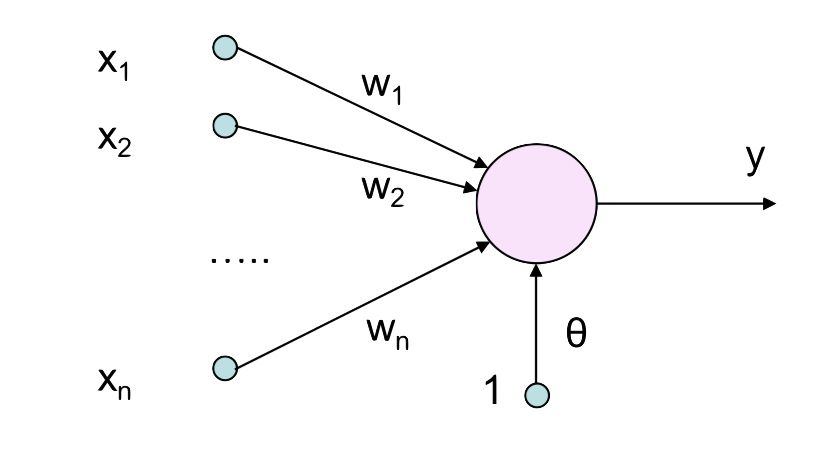
\includegraphics[scale=.35]{perceptron.jpg}}
\end{figure}

La salida de cada célula se calcula mediante:
$$y=\mathcal{F}\left(\sum_{i=1}^n x_i w_i+\theta\right) \quad \mathcal{F}(s) = \begin{cases}1 & \textit{si}\quad  x> 0\\-1 & \textit{en caso contrario}\end{cases}$$

La función escalón lo hace discriminante, si solo hay una célula y da 1 pertenece a la categoría A y si es -1 a la categoría B.

El número de células de un Perceptrón se corresponde con la dimensión de la entrada, y el número de células de salida, con el número de clases a discriminar.

En el caso binario, dos entradas una salida, el perceptrón representa una recta que divide el plano en dos partes cada una categoría.

\subsubsection{Aprendizaje}
El proceso de aprendizaje del perceptrón consiste en descubrir los parámetros de una recta que deje a todos los ejemplos de la clase A en un lado, y a los de la clase B en el otro.

Dado un conjunto de ejemplos de prueba distribuidos de los que se conoce su categoría, se trata de obtener la ecuación del hiperplano que deja a un lado los ejemplos de un tipo, y a otro los del otro.
$$A=(\vec{a}_1, ..., \vec{a}_n) \quad B=(\vec{b}_1, ..., \vec{b}_n)$$
$$\forall \vec{a} \in A,, w_1a_1+\cdot+w_na_n+\theta > 0$$
$$\forall \vec{b} \in B,, w_1b_1+\cdot+w_nb_n+\theta < 0$$
Para todos los puntos de A deben dar la misma categoría y los de B deben dar la otra.
\pagebreak

El proceso de aprendizaje necesita de un conjunto de ejemplos $\chi$ para los cuales tenemos una respuesta d($\chi$), y es un aprendizaje por refuerzo:
\begin{itemize}
	\item Si la red da una respuesta correcta, no se modifican los pesos.
	\item Si da una respuesta incorrecta, se modifican los pesos una cantidad fija.
\end{itemize}

El incremento de los pesos se realiza mediante la expresión: $\Delta w_i = d(\vec{x})x_i, , x \in \chi$

Si la \textbf{salida obtenida es y($\vec{x}$) = 1, y la deseada es d($\vec{x}$) = -1, entonces $w_i = -x_i$}. La salida es mayor que la esperada, y los pesos se decrementan

Si la \textbf{salida obtenida es -1, y la deseada es 1, entonces $w_i = x_i$.} La salida es menor que la esperada, y los pesos se incrementan.

\subsubsection{Validación}
Se realiza de forma iterativa.

\begin{enumerate}
	\item Inicialización aleatoria de los pesos y el umbral de la red.
	\item Se toma un ejemplo entrada-salida $\vec{x} = (x_1, x_2, ..., x_n), d(\vec{x})$
	\item Se calcula la salida de la red: $y(\vec{x}) = f (x_1w_1 + x_2w_2 + ... + x_nw_n + \theta)$
	\item Si $y(\vec{x}) \neq d(\vec{x})$ (clasificación incorrecta) se modifican los pesos y el umbral:
	
	Si $\vec{x} \in A, d(x) = 1 \rightarrow w_i(t+1) = w_i(t)+x_i, \theta(t+1) = \theta(t)+1$
	
	Si $\vec{x} \in B, d(x) = -1 \rightarrow w_i(t+1) = w_i(t)-x_i, \theta(t+1) = \theta(t)-1$

	\item Se vuelve al paso 2 hasta completar el conjunto de patrones de entrenamiento.
	\item Se repiten los pasos 2, 3, 4 y 5 hasta alcanzar el criterio de parada.
\end{enumerate}

Cada una de las capas representa una recta por eso en el problema XOR hacían falta más capas.

\subsubsection{Tasa de aprendizaje}
Es el ritmo con el que aprende, es un valor entre 0 y 1 que regula la variación de los pesos en cada iteración, para que no se vayan mucho y oscilen.

$$w_i(t+1)=w_i(t)+\gamma d(\chi)x_i$$

Se suelen empezar con valores mayores y se va reduciendo una vez se va aproximando (balance exploración-explotación)

\end{document}